%iffalse
\let\negmedspace\undefined
\let\negthickspace\undefined
\documentclass[journal,12pt,twocolumn]{IEEEtran}
\usepackage{cite}
\usepackage{amsmath,amssymb,amsfonts,amsthm}
\usepackage{algorithmic}
\usepackage{graphicx}
\usepackage{textcomp}
\usepackage{xcolor}
\usepackage{txfonts}
\usepackage{listings}
\usepackage{enumitem}
\usepackage{mathtools}
\usepackage{gensymb}
\usepackage{comment}
\usepackage[breaklinks=true]{hyperref}
\usepackage{tkz-euclide} 
\usepackage{listings}
\usepackage{gvv}                                        
%\def\inputGnumericTable{}                                 
\usepackage[latin1]{inputenc}                                
\usepackage{color}                                            
\usepackage{array}                                            
\usepackage{longtable}                                       
\usepackage{calc}                                             
\usepackage{multirow}                                         
\usepackage{hhline}                                           
\usepackage{ifthen}                                           
\usepackage{lscape}
\usepackage{tabularx}
\usepackage{array}
\usepackage{float}


\newtheorem{theorem}{Theorem}[section]
\newtheorem{problem}{Problem}
\newtheorem{proposition}{Proposition}[section]
\newtheorem{lemma}{Lemma}[section]
\newtheorem{corollary}[theorem]{Corollary}
\newtheorem{example}{Example}[section]
\newtheorem{definition}[problem]{Definition}
\newcommand{\BEQA}{\begin{eqnarray}}
\newcommand{\EEQA}{\end{eqnarray}}
\newcommand{\define}{\stackrel{\triangle}{=}}
\theoremstyle{remark}
\newtheorem{rem}{Remark}

% Marks the beginning of the document
\begin{document}
\bibliographystyle{IEEEtran}
\vspace{3cm}

\title{Subjective questions}
\author{AI24BTECH11018 - Sreya}
\maketitle
\newpage
\bigskip
\begin{enumerate}

    

\renewcommand{\thefigure}{\theenumi}
\renewcommand{\thetable}{\theenumi}
\item[21.] Sketch the curves and identify the region bounded by $x=\frac{1}{2}$,$x=2$,$y=\ln{x}$ and $y=2^x$. Find the area of region.

\hfill{($1991-4 Marks$)}

\item[22.] if $f$ is a continous function with $\int_{0}^{x}f(t)dt\rightarrow\infty$ as $\mid x \mid\rightarrow\infty$, then show that every line $y=mx$\\
\begin{figure}[h!]
    \centering
    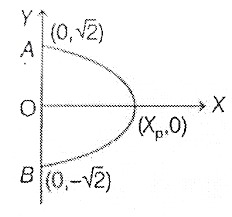
\includegraphics[width=\linewidth]{image.jpg}
    \label{figure1}
\end{figure}\\
intersects the curve $y^2+\int_{0}^{x}f(t)dt=2!$

\hfill{$1991-4 Marks$}\\

\item[23.] Evaluate $\int_{0}^{\pi}\frac{xsin2xsin(\frac{\pi}{2}cosx)}{2x-\pi}$

\hfill{$1991-4 Marks$}

\item[24.]  Sketch the region bounded by the curves\\ $y=x^2$ and
$y=\frac{2}{1+x^2}$. Find the area.


\hfill{$1992-4 Marks$}

\textbf{25.} Determine a positive integer $n\leq 5$, such that $\int_e^x(x-1)^n=16-6e$

\hfill{\textcolor{black}{($1992-4 Marks$)}}\\

\item[26.]  Evaluate $\int_{2}^{3}\frac{2x^5+x^4-2x^3+2x^4+1}{(x^2+1)(x^4-1)}dx$

\hfill{\textcolor{black}{($1993 - 5 Marks$)}}

\item[27.]  Show that $\int_{0}^{n\pi+v}\mid sinx \mid dx=2n+1-cosv$ where n is a positive integer and $0 \leq v < \pi$

\hfill{\textcolor{black}{($1994-4 Marks$)}}\\

\item[28.]  In what ratio does the x-axis divide the area of the region bounded by the parabolas $y=4x-x^2$ and $y=x^2-x$?

\hfill{\textcolor{black}{($1994-5 Marks$)}}\\

\item[29.]  $I_m=\int_{0}^{\pi}\frac{1-cosmx}{1-cosx}dx$. Use mathematical induction to prove that $I_m=m\pi$, $m=0,1,2,3,......$

\hfill{\textcolor{black}{($1995-5 marks$)}}\\

\item[30]  Evaluate the definite integral:
$\int\limits_{\frac{-1}{\sqrt{3}}}^{\frac{1}{\sqrt{3}}}(\frac{x^4}{1-x^4})cos^{-1}(\frac{2x}{1+x^2})$

\hfill{\textcolor{black}{($1995-5Marks$)}}\\

\item[31.]  Consider a square with vertices at (1,1),(-1,1),(-1,-1) and (1,-1). Let s be the region consisting of all points inside  the square which are nearer to the orgin than to any edge. Sketch the region S and find its area.

\hfill{\textcolor{black}{($1995-5 Marks$)}}\\

\item[32.]  Let $A_n$ be the area bounded by the curve\\ $y=(tanx)^n$ and the lines $l=0$,$y=0$ and $x=\frac{\pi}{4}$. Prove that for $n>2$, $A_n+A_n-2=\frac{1}{n-2}$ and deduce\\ $\frac{1}{2n+2}<A_n<\frac{1}{2n-2}$.

	\hfill{\textcolor{black}{($1996-3 Marks$)}}\\

\item[33.]  Determine the value of $\int_{-\pi}^{\pi}\frac{2x(1+six)}{1+cos^2x}dx$.\\


\hfill{\textcolor{black}{($1997-5 Marks$)}}

\item[34.]  Let $f(x)$= Maximum {$x^2,(1-x)^2,2x(1-x)$}, Where $0 \leq x \leq 1$. Determine the area of the region bounded by the curves $y=f(x)$,x-axis,$x=0$ and $x=1$.
\hfill{($1997-5 Marks$)}
\item[35.]  Prove that $\int_{0}^{1}tan^{-1}(\frac{1}{1-x+x^2})dx$=2$\int_{0}^{1} tan^{-1}xdx$. Hence or otherwise, evaluate the integral $\int_{0}^{1}tan^{-1}(1-x+x^2)dx.$
\hfill{($1998-8 Marks$)}
\end{enumerate}


\end{document}
